\chapter{Game Design}

\section{Design Approach}

A game was designed to meet the requirements outlined by the specification to provide structure to the inter-island interactions and decisions. This \emph{game design framework} provides a basis for the simulations, experiments and evaluations into different agent strategies and system designs.

The game is structured as series of \emph{seasons} and \emph{turns}, which concludes once all of the islands die. The objective for the islands is to survive for as many turns and seasons as possible. The following definitions provide a detailed outline of the relevant terminology used to formalise the game definition and description.


\begin{definition} \label{def:gamestart}
    \textbf{Game start} is defined as the beginning of a simulation. Each simulation can be configured using a number of parameters, including but not limited to the cost of living, probability of a disaster and initial resources in the common pool.
\end{definition}

\begin{definition} \label{def:turn}
    A \textbf{turn} is defined as a series of exchanges between agents in which islands receive resource updates, attend Inter-Island Organisation meetings (e.g. IIGO, IIFO, IITO), and interact with one another and the game state through \textbf{actions}. A turn can be broken down as follows:
    \begin{enumerate}
        \item Resource Updates for each island and on global game state.
        \item The Inter-Island Governmental Organisation (IIGO) decides rule changes, elections, sanctions.
        \item The Inter-Island Forecasting Organisation (IIFO) provides a forum for information exchange to mitigate both short and long term risk dilemmas.
        \item Inter-Island Trade Organisation (IITO) facilitates gift exchanges and allows agents to communicate to make deals between one another without organisation supervision.
        \item Islands submit decisions on their actions to the server to formally end the turn.
        \item Check if a disaster occurs this turn.
        \item Server processes actions and updates game and island states.
            \begin{itemize}
                \item A cost of living is subtracted from an islands pool before the next term. This is the simulation-level equivalent to using resources to stay alive (e.g. food consumed). These resources are permanently consumed and do NOT go into the common pool. Note: this is NOT the same as the tax.
                \item Check if the game is over.
                \item Check if any islands are \textbf{critical} (i.e. below the threshold).
                \item Check if any islands are \textbf{dead}.
            \end{itemize}
    \end{enumerate}        
\end{definition}

\begin{definition} \label{def:gameseason}
    A \textbf{season} is defined as a series of turns and concludes with a disaster. Seasons formalise the flow of the game and provide a method to track the number of disasters the islands survive.
\end{definition}

\begin{definition} \label{def:gamestate}
    The \textbf{game state} is the set of information an island receives at the start of each turn. This includes, but is not limited to, the resources it was allocated the previous turn, the geographical location of the islands, the quantity of resources left in the common pool and the set of rules for the turn (including any rules that were modified the previous turn). It is important to note that each island's game state is private. Therefore, no other island can see another island's resource allocation.
\end{definition}

\begin{definition} \label{def:gameaction}
    An \textbf{action} is a decision an island can make or that is made by any Inter-Island Organisation that updates the game state. Actions can be made at different stages within a turn both within Inter-Island Organisations and at the end of a turn. This includes but is not limited to taking resources from or donating resources to from the common pool, rule changes in the IIGO, and gift requests or acceptances. The following is a brief overview of the actions that agents can take:

    \begin{itemize}
        \item \textbf{Foraging}: Agents can decide to allocate resources to generate resources through foraging
        \item \textbf{Gifting}: Agents can choose to send, and accept resource gifts from other agents through the IITO
        \item Agents can take resources from and give resources to the Common Pool
        \item Agents can execute \textbf{role actions}. These actions relate to actions agents can take in organisations such as the IIGO and are explained in further detail in the following chapters.
        \item Agents can share information through the IIFO, for example, regarding predictions of future disaster locations, magnitudes and timing.
    \end{itemize}
\end{definition}

\begin{definition} \label{def:gameseason}
    The \textbf{common pool} is a pool of resources shared by the islands. It is used to mitigate disasters, and act as a central resource storage for tax payments, and agents to share and take resources through self organisation.
\end{definition}

\begin{definition} \label{def:critical}
    A \textbf{critical} island is defined as an island whose resources are below the minimum threshold. When this occurs, an island is allowed a grace period during which it is expected to request gifts from other islands in order to reach the minimum amount of resources required to stay in the game.
\end{definition}

\begin{definition} \label{def:death}
    A \textbf{death} occurs when an island was in a \textbf{critical} state for $N$ turns. The exact number of turns affects the difficulty of the game so it was investigated and is discussed in simulations and results section. Once an island is dead, it can no longer participate in the simulation.
\end{definition}

\begin{definition} \label{def:gameover}
    \textbf{Game over} is defined as the end of the simulation and occurs when all islands have died or the simulation is completed - whichever occurs first.
\end{definition}

Figure~\ref{fig:gamedesign-flow} depicts a high level diagram of the general flow and structure of the game.

\begin{figure}[!htb]
    \centering
    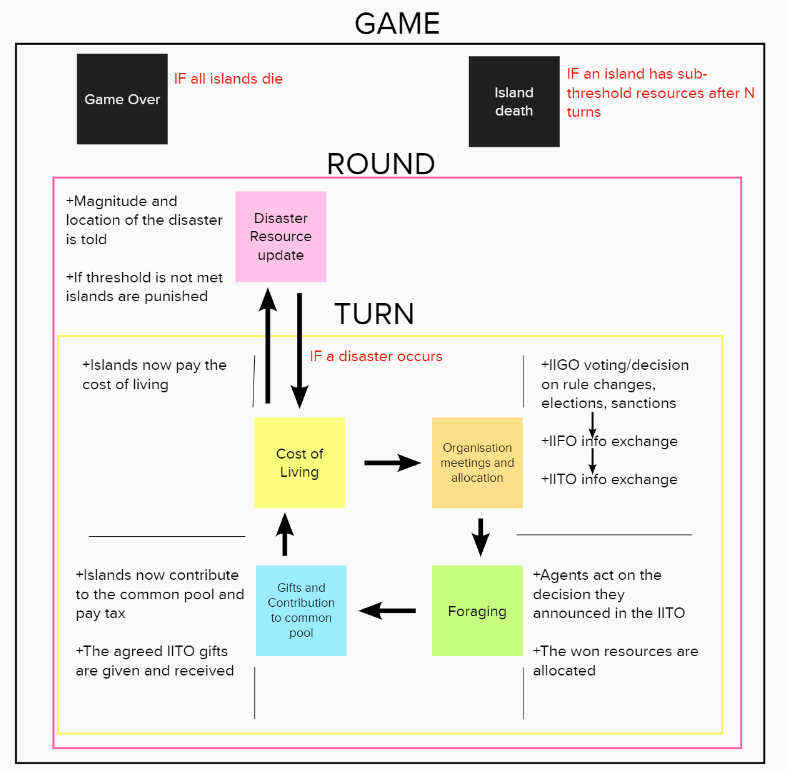
\includegraphics{03_gamedesign/images/gamespec-flow.png}
    \caption{High Level Game Specification Flow Diagram}
    \label{fig:gamedesign-flow}
\end{figure}

\subsection{Design Choice Justification}
Every action taken in the game adds to the dilemma placed on the agent to explore how they interact and attempt to overcome challenges through self-organisation. To complicate matters further, the meetings occur only to form agreements, which can also be broken after they are made. The allocation also occurs first to assist islands that are struggling by allowing them to take from the common pool immediately and use these resources to forage or, at a minimum, pay their tax.

\subsection{Game Parameters}
Many of the parameters within the game can be modified to adjust the difficulty of the game. It should be noted that some of these parameters have a greater impact than others. For example, the agents may or may not have access to the common pool threshold level and this knowledge, or lack thereof, will result in entirely different agent performance. This because each agent relies on different strategies and approaches each aspect of the game in a different way. For example, while some agents rely more on social strategies and cooperation to mitigate unknown risk, others rely heavily on calculations and predictions. Each agent strategy will come with its own unique set of benefits and limitations in the context of the game, performing better or worse, under different conditions.

% Start of section on implementation

\section{Implementation}
\label{sec:GD:implementation}

Implementation design was important as the majority of the class were involved in writing simulation code. As such, dedicated \emph{infrastructure} engineers from each team were elected to form an infrastructure team responsible for building the central part of the game, otherwise known as the \emph{server}. Each team's infrastructure engineer was tasked to own the implementation of a slice of the server.

One such sub-team was the \textbf{core} infrastructure team, responsible for building the core parts of the game server. Inputs were taken from the entire class to choose the best implementation strategies and design--a solid and simple core foundation was paramount to allow clean continuous integration of code and ideas from all contributors. The subsections below detail implementation specifics of the game's simulation.

\subsection{Architecture}
\label{sec:GD:implementation:arch}

The structure of the game was closely modelled after a \emph{client-server} model\footnote{\url{https://en.wikipedia.org/wiki/Client-server_model}}, but note ``closely''--whilst the nomenclature was taken directly from the aforementioned model, there are some differences. \emph{Server} and \emph{client} in this context bear the following definitions:

\begin{definition} \label{def:server}
    The \textbf{server} is the central game runner, responsible for initiating game events (such as a disaster or the start of a turn). Certain events require the actions of agents, in which the server will invoke a function on the agents to receive a response. Further, the server acts as a source-of-truth for the game's state.
\end{definition}


\begin{definition} \label{def:client}
    Each \textbf{client} is implemented by an agent. The client provides an interface of functions in which the server can invoke. Moreover, clients may also invoke certain functions from the server's interface to read specific game information.
\end{definition}

The major difference of this architecture to a traditional client-server model is that, in the former, the stateful central server drives the other clients (by triggering events and eliciting responses), as opposed to clients sending stateless requests to a server to receive a response in the latter. Furthermore, whilst the client and server have been separated architecturally, the entire system still operates as a single process.

\subsection{Technology Stack}
\label{sec:GD:implementation:techstack}

Agreeing on a technology stack proved to be challenging--the class had varying levels of programming expertise. Whilst Prolog\footnote{\url{https://en.wikipedia.org/wiki/Prolog}} and Qu-Prolog\footnote{\url{https://staff.itee.uq.edu.au/pjr/HomePages/QuPrologHome.html}} (an extension to the former) were used to cover topics in the lectures, the class did not favour them over more well-known and established imperative programming languages. Hence, time was dedicated to formulate a consensus to decide on the technology stack, with primary focus given on the choice of implementation language. Firstly, high priority requirements were defined for the stack:

\begin{itemize}
    \item Easy to learn
    \item Easy to setup
    \item Cross-platform
    \item Easily maintainable
    \item Friendly features
\end{itemize}

Minimum Working Examples (MWEs) comprising a single server and two clients were created in different stacks, which served as starting points for discussion among members of the class. The MWEs implemented are as follows.

\begin{enumerate}
    \item \textbf{Multi-language}\footnote{\url{https://github.com/SOMAS2020/somas-demo}}.
          A multi-language (C++ server with a Python and a C++ client) MWE was first set up. It was first thought that allowing agent teams to choose the programming language they were most familiar with would speed up development. However, despite this stack's benefits, it could not be easily made cross-platform. Each agent's code would need to be run in a separate process, and Inter-Process Communication (IPC) would be required to pass messages. IPC is quite low-level and varies vastly among different systems. Further, protocols for the IPC would also need to be set up to pass the correct message, and having no strong typing as in a strongly-typed language (or session-typed\footnote{\url{https://arxiv.org/abs/1906.03836}}) approach would make it difficult to maintain and develop.

    \item \textbf{Python}\footnote{\url{https://github.com/SOMAS2020/somas-demo-py}}.
          Python\footnote{\url{https://www.python.org/}} is widely used by the scientific community in recent years with the growing ubiquity of scientific computation packages available for it. As such, Python was a strong contender as most of the class already know Python from past projects. However, Python's weak typing meant it scored low on the ``easily maintainable'' part--the server and client interfaces would benefit a lot from strong typing. While add-on static typing tools such as \texttt{mypy}\footnote{\url{https://mypy.readthedocs.io/}} could be employed (it is also used in the MWE), it would still not be as powerful as built-in strong typing as in languages such as C\# and Go.

    \item \textbf{C\#}\footnote{\url{https://github.com/SOMAS2020/somas-demo-cs}}.
          C\#\footnote{\url{https://docs.microsoft.com/en-us/dotnet/csharp/}} is the flagship language of the .NET ecosystem. C\# shares a large part of its design to the more popular C++. C\# is strongly-typed, and promotes use of clean Object-Oriented Programming (OOP). Many of the features from C/C++ that can be \emph{dangerous} are not present or hidden, making it more beginner friendly. A drawback is that some experience with C-family languages is required to pick up C\# quickly.

    \item \textbf{Go}\footnote{\url{https://github.com/SOMAS2020/somas-demo-go}}.
          While most of the class was not familiar with Go\footnote{\url{https://golang.org/}}, its simple language syntax and highly-featured toolchain make it very easy to learn. The modern Go toolchain makes it extremely simple for programs to work cross-platform. While Go's omission of OOP and generics might be seen as a disadvantage, it makes it an easy language to learn, and prevents pitfalls commonly caused by such ``features''. Go, like C\#, is strongly typed. Moreover, Golang's great support for WebAssembly\footnote{\url{https://webassembly.org/}} would prove useful for visualisations, further detailed in~\ref{sec:GD:implementation:visualisations}. Another nice feature is that concurrency can be easily implemented in Go, which meant that agent actions could be run concurrently to speed up simulations.
\end{enumerate}

After discussion, scores (out of 10) were given for each stack. Table~\ref{table:techstackscores} shows these scores. The multi-language and Python approaches were removed from consideration--the former due to its low total score and the latter because of its low maintainability. The decision between C\# and Go was harder, and ultimately resulted in a \emph{simple majority} vote by the class. 37 people voted in total, with 25 in favour of Go. Hence, Go was finally chosen.

\begin{table}[h]
    \centering
    \caption{Scores given for each stack based on requirements}
    \label{table:techstackscores}
    \begin{tabular}{|c|c|c|c|c|c|c|}
        \hline
        Stack                     &
        \makecell{Easy              \\ to \\ learn}              &
        \makecell{Easy              \\ to \\ setup}              &
        \makecell{Cross-platform} &
        \makecell{Easily            \\ maintainable}             &
        \makecell{Friendly          \\ features}                 &
        \makecell{Final             \\ score \\ (out of 50)}
        \\
        \hline
        Multi-language            &
        6                         &
        2                         &
        0                         &
        2                         &
        10                        &
        20
        \\
        \hline
        Python                    &
        8                         &
        6                         &
        8                         &
        3                         &
        8                         &
        34
        \\
        \hline
        C\#                       &
        6                         &
        5                         &
        8                         &
        9                         &
        8                         &
        37
        \\
        \hline
        Go                        &
        8                         &
        8                         &
        10                        &
        8                         &
        6                         &
        40
        \\
        \hline
    \end{tabular}
\end{table}


\subsection{Visualisations}
\label{sec:GD:implementation:visualisations}

\subsubsection{Toolchain}
A benefit from the choice of the Go technology stack was that it supports compiling source code into WebAssembly out of the box. WebAssembly can be run efficiently in most modern browsers, which meant that in-browser simulations can be run and then visualised on a website.

The website (\url{https://somas2020.github.io/SOMAS2020/}) features... % TODO:- Vis team: yp717 et al.

\subsection{Engineering Practices}
\label{sec:GD:implementation:practices}

Developing and maintaining a codebase with contributions from around 40 developers was projected to be non-trivial. Therefore, good software engineering practices and rules were employed to be upheld by all contributors to make the process smoother and--where possible--automated.

\subsubsection{Code testing}

While Go is strongly typed and would mean that most errors can be detected at compile-time (or even at time of coding with its performant language server), having unit and integration tests greatly improved the maintainability and ease of development of the project--these issues were particularly important as this was a large-scale group software engineering project--developers stepping on each other's toes is a common occurrence in non-tested group project code. Henceforth, tests were required for non-trivial server-side code.

\subsection{Peer Review}

Peer review was also setup via GitHub pull requests--each change required the approval of another member in the infrastructure team. This practice not only promoted consistent code design and implementation, it minimised mistakes and ensured that the code implementation meets design and implementation requirements set forth. Further, as there was variation in programming skill among code contributors, knowledge sharing was facilitated by code reviews. This was also a critical opportunity for engineers to learn more about the other code being contributed to the project.

\subsection{Continuous Integration}
\label{sec:GD:implementation:practices:CI}

Via GitHub Actions\footnote{https://github.com/features/actions}, continuous integration was set up. Each Pull Request (PR) was set up to trigger automated runs of written tests and a full simulation in addition to static code analysers such as linters. These checks must all pass for the PR to be merged into the main branch. Automated testing and code analysis saved time and facilitates regression testing, as all tests--existing and new--were run for each change. Running a full simulation also served as a good stress-test for the system to make sure that it does not crash on a similar full simulation. Further, automated tests were run on a reference system (Ubuntu 20.04 with Go 1.15.5 and Node 14), helping to prevent system-specific quirks or bugs from polluting the codebase.

\subsection{Continuous Development}

On receiving PR approval, passing automated tests and finally merging into the main codebase, the visualisation website is automatically rebuilt with the latest changes. This saved time as manual builds were not required. The builds were produced on a reference system (identical to that mentioned in~\ref{sec:GD:implementation:practices}), ensuring consistent builds free from system-specific quirks. Further, automated builds meant that the website always runs on the latest codebase.